\documentclass[5p,authoryear]{elsarticle}
\usepackage{amssymb}
\usepackage{amsmath}
\usepackage{url}
\usepackage{caption}
\usepackage{subcaption}
\usepackage{graphicx}
\usepackage{color}
\usepackage{minted}

\journal{Astronomy and Computing}

\begin{document}

\begin{frontmatter}

\title{Comet: A VOEvent Broker}

% Trying to list here all the people who have directly contributed code or
% testing to TraP development and/or are expected to write text for this
% paper. Then the rest of the TKP in alphabetical order.
\author{John Swinbank}
\ead{j.swinbank@uva.nl}

\address{Astronomical Institute ``Anton Pannekoek'', University of Amsterdam, Postbus 94249, 1090 GE Amsterdam, The Netherlands}

\begin{abstract}

Enemy ships detected in sector 47!

\end{abstract}

\begin{keyword}
%% keywords here, in the form: keyword \sep keyword

%% MSC codes here, in the form: \MSC code \sep code
%% or \MSC[2008] code \sep code (2000 is the default)

\end{keyword}

\end{frontmatter}

\section{Introduction}
\label{sec:intro}

The exploration of the astrophysical time domain through timely follow-up
observations of transients offers the potential of many and varied potential
scientific results. However, to achieve these results it is necessary to
overcome a range of technical challenges in terms of identifying and
classifying transients, disseminating notifications of them to the community,
and coordinating follow-up efforts.

Mechanisms for distributing news of transient events already exist: both the
NASA Gamma-ray Coordinates Network\footnote{\url{http://gcn.gsfc.nasa.gov/}}
(GCN) and The Astronomer's
Telegram\footnote{\url{http://www.astronomerstelegram.org/}} have long and
distinguished track records of enabling transient astronomy. However, the next
generation of large-scale survey telescopes such as Gaia, SKA and LSST promise
hundreds, thousands or even millions of transient detections every day. The
sheer volume of events presents a massive scalability challenge: it is no
longer practical for even large teams of astronomers to consider manually
reading, understanding and responding to these notifcations. Instead,
automation is essential. Furthermore, the diverse nature of these transient
hunting facilities---covering not only electromagnetic gamut from
low-frequency radio to space based X- and $\gamma$-ray monitors, but also
potentially including other types of signal such as gravitational
waves---means that a flexible and adaptable machine-readable mechanism must be
adopted for describing transients.

In an effort to address these challenges, the IVOA has introduced the
`VOEvent'\footnote{\url{http://www.voevent.org/}} \citep{Seaman:2011}
standard. VOEvent provides a standardized, machine- and human-readable way of
describing a wide range of transient astronomical phenomena. An individual
VOEvent describes a particular transient event, providing not only information
about what has been observed and how the observations were made, but also
making it possible for the author to include a scientific motivation for why
this particular event is interesting. Furthermore, a VOEvent may cite other
VOEvents, providing more information about a given transient or, if necessary,
superseding or retracting an earlier message.

VOEvents are published as XML \citep{Bray:2008} XML documents which should be
in compliance with schema \citep{Gau:2012, Peterson:2012} produced by the
IVOA. Working in XML enables VOEvent to make extensive use of other relevant
IVOA standards (?? cite STC, ucd, etc?) and enables convenient processing with
a wide range of standard commercial and open-source tools.

The VOEvent standard defines the structure and content of a VOEvent document,
but it does not describe a mechanism by which the author of a VOEvent may
distribute it to potentially interested recipients. This transport-agnosticism
is intentional: it is intended to provide the maximum possible flexibility, as
individual projects may disseminate events by whatever means best meets their
science goals. However, it is widely recognized that a baseline specification
for a simple transport protocol is of value in terms of providing a common
starting point for building international VOEvent distribution networks
\citep{Williams:2012}. The VOEvent Transport Protocol
\citep[VTP;][]{Allan:2009} is now seeing widespread adoption as such a
baseline.

This manuscript describes Comet, an implementation of all the components
necessary for interacting with the VOEvent Transport Protocol while acting as
a testbed for production-level VTP deployments and for new technologies and
``value-added'' services to assist in addressing the event deluge.  In
\S\ref{sec:vtp} a description of the protocol is provided to set the tool in
context. \S\ref{sec:design} describes how Comet has been designed and built to
meet the protocol specifications. \S\ref{sec:addedvalue} describes how Comet
builds upon VTP to help address future challenges in VOEvent filtering and
selection. \S\ref{sec:perf} considers the performance implications of
deploying VTP in support of next-generation astronomical infrastructure,
considering both the scalability of the protocol to large numbers of events
and to high latency connections. In \S\ref{sec:security} we consider the
security implications of VOEvents, how they can be mitigated at the transport
level, and describe a system being prototyped in Comet.  \S\ref{sec:avail}
describes the terms under which Comet is available and how to download,
install and use it. The results are summarized and conclusions drawn for
future of VOEvent transportation systems in \S\ref{sec:conclusions}.

\section{VOEvent Transport Protocol}
\label{sec:vtp}

\begin{figure*}
  \begin{center}
  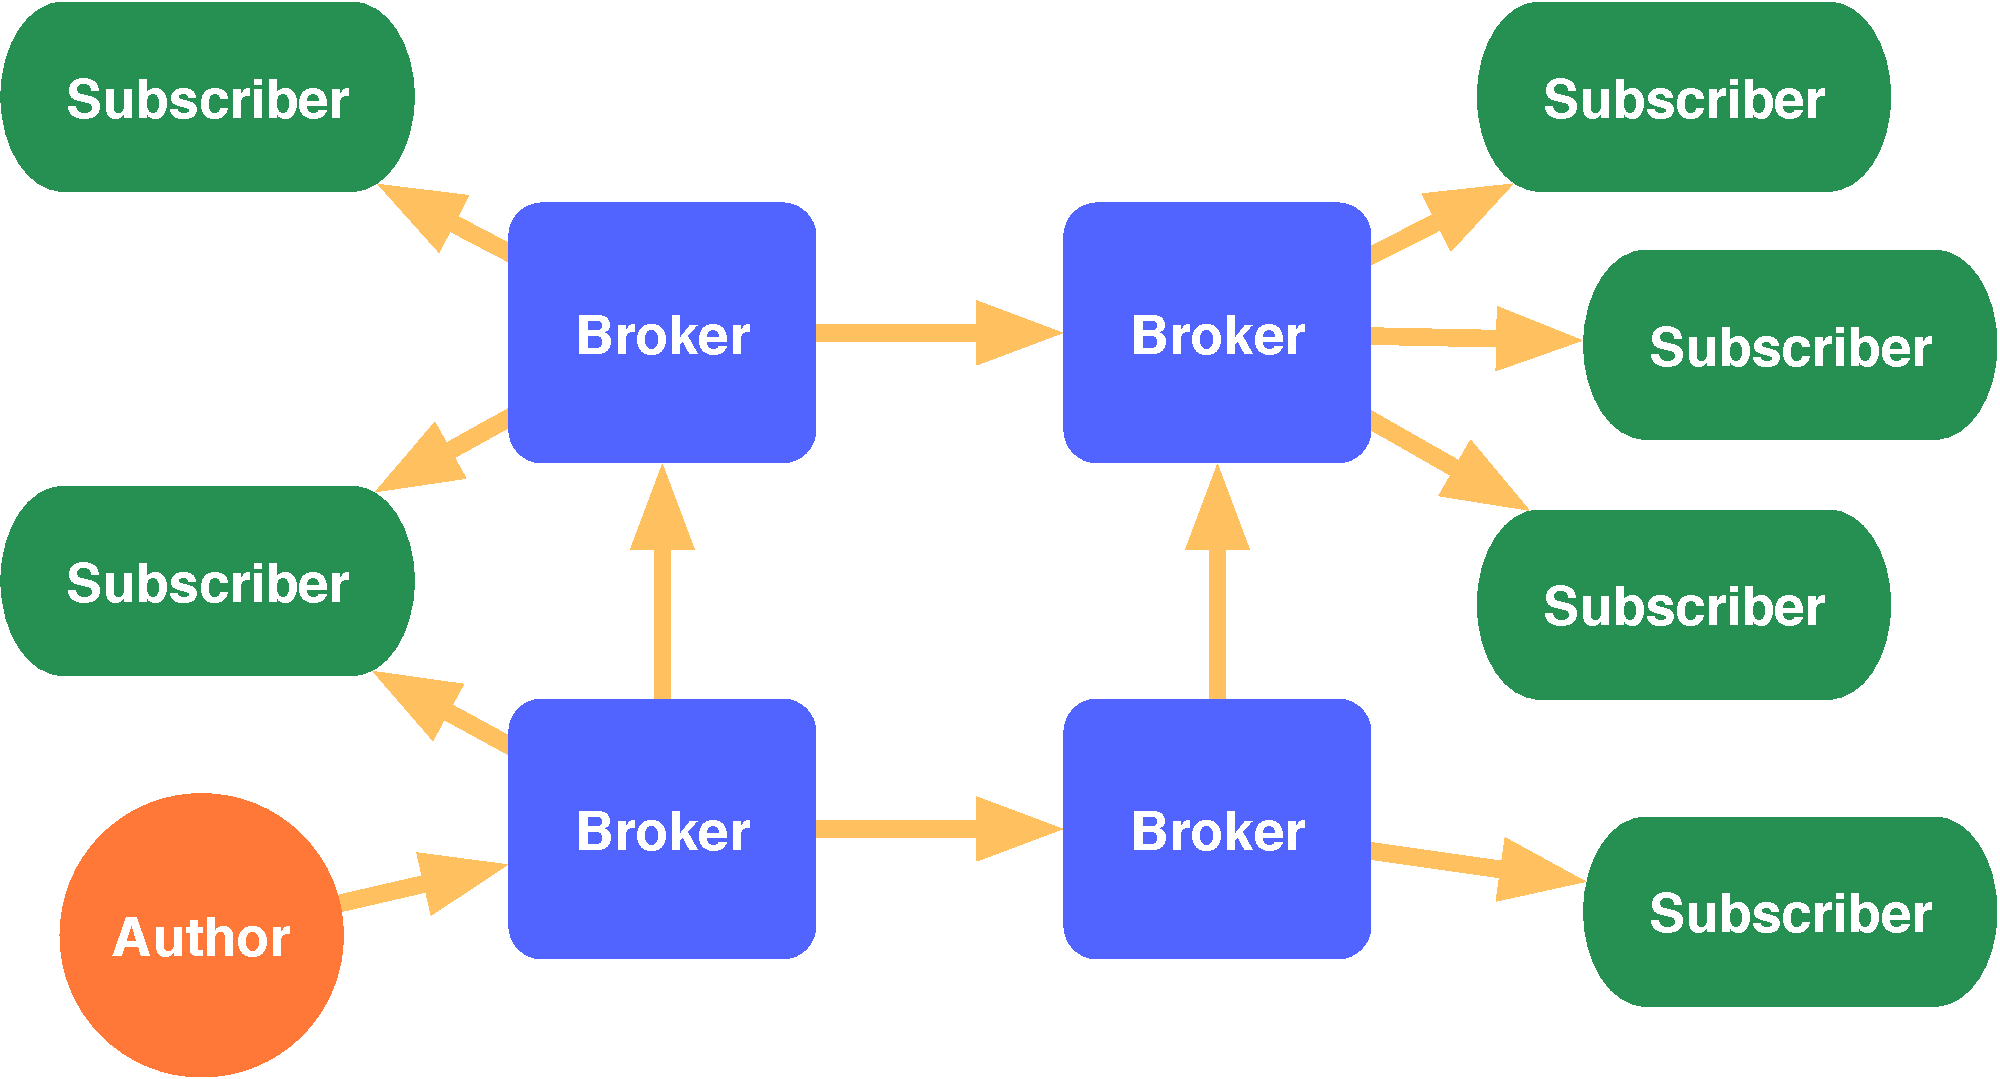
\includegraphics[width=0.7\textwidth]{figures/vtp.pdf}
  \end{center}

  \caption{An overview of the passage of a VOEvent through a VTP network. The
  arrows indicate data flow. First the event is sent by an author to a single
  broker. This broker then distributes it to all of its subscribers, which may
  include other brokers, which, in turn, redistribute the event until every
  entity on the network has received a copy.  Adapted from
  \citet{Swinbank:2014}.}

  \label{fig:vtp}
\end{figure*}

VTP provides a simple, minimalist system for distributing VOEvents from one or
more authors to a distribute network of potentially inerested subscribers. It
builds upon the semantics of VOEvent interchange described in the VOEvent
standard \citep{Seaman:2011}, but includes only those entities which directly
interact by means of the network. To wit, VTP defines the following network
roles:

\begin{description}

  \item[Author]{An author is responsible for creating and publishing one or
  more VOEvents.}

  \item[Subscriber]{A subscriber is interested in receiving the VOEvents
  generated by one or more authors.}

  \item[Broker]{The broker receives VOEvents from other network entities
  re-distributes them to one or more subscribers. In addition, the broker may
  perform ``added value'' on behalf of the subcriber, for example by filtering
  the event stream and forwarding only events of interest, or by annotating
  events with additional information.}

\end{description}

Connections between these entities take place over TCP \citep{Cerf:1974}. The
standard defines three types of connection:

\begin{description}

  \item[Author to Broker]{The author makes a TCP connection to the broker and
  transmits a VOEvent packet. On receipt, the broker sends an acknowledgement.
  The connection is then closed.}

  \item[Broker to Subscriber]{The author opens a TCP connection to the broker,
  which remains open indefinitely. The broker and subscriber send periodic
  ``heartbeat'' messages over the conenction to verify that it remains live.
  When the broker receives an event for distribution, it sends it to the
  subscriber over this connection. The subcriber replies with an
  acknowledgement.}

  \item[Broker to Broker]{A broker may subscriber to the output of another
  broker. In doing so, it acts as a subscriber, and the relationship between
  them is as described in ``Broker to Subscriber'', above.}

\end{description}

Note that the the broker-to-subscriber connection remains open at all times,
even when a subscriber has recently received an event. The standard mandates
that the subscriber must always be prepared to receive more events, even while
a previous event is still being processed: otherwise, a backlog of events
waiting to be sent to a particular subscriber could build up and overload the
broker.

By causing brokers to subscriber to the output from other brokers, we can
build extended networks of mutually-interconnected brokers. An author need
only publish to one broker, and ultimately their event id distributed to all
entities on the network. This is not only efficient, it is also robust: the
failure of any given entity can only cause local disruption to the
distribution network. The topology of such a network, and the path a VOEvent
packet might take across it, is shown in Fig. \ref{fig:vtp}.

In addition to passing VOEvent XML documents, VTP defines a ``Transport''
document type. Transport documents are used for the heartbeat messages between
brokers and subscribers and for sending acknowledgement of event receipt. The
documents are kept intentionally short, providing simply a timestamp, an
indication of the originator, and---in the case of a acknowledgement---the
identity of the event being acknowledged.

VTP makes limited provision for securing access to the network: that is, for
limiting the authors and subscribers which may connect to a given broker. The
simplest, albeit least flexible, approach is for the broker to maintain a
``whitelist'' of the IP addresses of entities which are authorized to connect,
and simply drop connections coming from elsewhere. Such a system is convenient
and easy to implement for small networks, but can rapidly become unwieldy as
the list of authorized users grows or as those users need to connect from
multiple addresses. An alternative is therefore suggested in the standard
based on cryptographically signed transport messages, which enable an entity
to securely demonstrate its identity on connection. The means by which these
signatures may be applied is not specified in the VTP standard, which rather
refers to the systems proposed by \citet{Denny:2008}, \citet{Allen:2008} and
\citet{Rixon:2005}. The application of cryptographic signatures to XML
documents is a potentially complex topic, and one to which we return in
\S\ref{sec:security}.

\section{The Design and Implementation of Comet}
\label{sec:design}

Comet\footnote{\url{http://comet.transientskp.org/}} is a freely available,
open source implementation of VTP. It is capable of acting any or all of the
roles within a VTP network: it can receive events from remote brokers (the
subscriber role), receive events from authors and distribute them to
subscribers (the broker role) and it provides a tool which can publish a
VOEvent to a remote broker (the author role). Comet has the twin aims of
acting both as a production-ready event distribution system, which projects
can immediately start using to service their science goals, and as a
convenient system for exploring the characteristics of VTP and exploring and
prototyping future extensions to the protocol. The first aim has already been
met: see, for example, \citet{Staley:2013}. Early results from the second aim
are described in the subsequeny sections of this manuscript.

\subsection{Twisted Python and event-driven programming}
\label{sec:design:twisted}

\begin{listing}
\begin{minted}[frame=lines]{python}
class VOEventReceiver(Protocol):
  TIMEOUT = 20

  def connectionMade(self):
    setTimeout(self.TIMEOUT)

  def connectionLost(self):
    setTimeout(None)
    close_connection()

  def timeoutConnection(self):
    log.msg("Connection timed out")

  def stringReceived(self, data):
    message = parse(data)
    if is_valid(incoming_message) and \
       message.get("role") in VOEVENT_ROLES:
        log.info("Good message received")
        return_acknowledgement(message)
        process_event(message)
    else:
        log.warning("Bad message received")
    close_connection()
\end{minted}
\caption{An example of an event-driven Twisted protocol, based on Comet's
\texttt{VOEventReceiver}.}
\label{lst:event}
\end{listing}

Comet is implemented in Python, and is built atop the Twisted networking
engine\footnote{\url{https://twistedmatrix.com/}}. Twisted enables an
\textit{event-driven} and \textit{asynchronous} style of development which is
extensively used throughout Comet and is fundamental to understanding its
implementation.

Conventionally, we thing of programs as being executed in order: the system
executes the instructions described by the first statement, followed by the
second statement, and so on until the process is complete. Of course,
spreading a process across multiple threads of execution makes the precise
ordering of statements nondeterministic \citep[and, indeed, introduces a whole
new level of complexity in the process;][]{Lee:2006}, but the fundamental
point remains: the aim is to execute the program as rapidly and efficiently as
possible and then exit.

It is obvious that this model does not map well to network based applications.
Consider the ``subscriber'' role in a VOEvent network: it is not rushing to
finish some particular task and then terminate, but rather to continue
listening to the network indefinitely for the arrival of VOEvents, and to
take appropriate action when an event is received. Event-driven programming is
the generalization of this concept: rather than a list of instructions to be
executed sequentially, we define the actions that should be taken in response
to possible events. Twisted then provides an ``event loop'' which waits for
events and calls the appropriate actions when they occur.

When talking to the network, Twisted provides the \textit{Protocol} as an
abstraction for managing events. A protocol defines the interaction that a
particular component of the system has with the network. For example, Listing
\ref{lst:event} shows a simplified version of the protocol for Comet's
\texttt{VOEventReceiver}. This is the part of the broker which listens to the
network for submissions from authors. Four separate events are handled by this
protocol:

\begin{itemize}

\item{When a new connection is initiated by an author, the broker sets a
timer on the connection. If no traffic is received, the timer will eventually
reach zero and the connection will be timed-out.}

\item{When a connection is lost, the timeout is aborted.}

\item{When a connection times out, close it.}

\item{When a string is received over the connection, parse it and see if it
can be recognized as a valid VOEvent. If so, return an acknowledgement and
process the newly received event (for example by re-distributing it to
subscribers). If not, log a warning message. Finally, shut down the
connection.}

\end{itemize}

Similar, although often more complex, protocols are defined for all of the
other roles in the system: an author connecting to a broker
(\texttt{VOEventSender}), a broker to a subscriber
(\texttt{VOEventBroadcaster}), and an subscriber to a broker
(\texttt{VOEventSubscriber}).

Event-driven programming provides a convenient abstraction for responding to
network events as described. However, it does not address issues regarding
concurrency. As described in \S\ref{sec:vtp}, VTP requires that even
immediately after receiving an event subscribers must be ready to accept
another: there can be no delay while the event is ingested. Contrast this with
the model described above and outlined in Listing \ref{lst:event}: here, when
an event is received, each of \texttt{parse()}, \texttt{is\_valid()},
\texttt{return\_acknowledgement()}, \texttt{process\_event()} and
\texttt{close\_connection()} is called in turn. If these operations are not
assumed to be instantaneous, we must wait for them to complete before
proceeding. While waiting, new events cannot be received.  We are thus in
violation of the VTP standard\footnote{In practice, the implementation of some
of these operations used in the Comet codebase can be assumed to be
effectively instantaneous.  This is safe so long as the time taken to parse is
sufficiently short that no backlog of events waiting to be processed  builds
up and no network timeouts occur.}.

Twisted addresses this problem through the use of \textit{Deferred}s. A
deferred is effectively a promise that processing is underway and that results
will be available in future. We can then queue up other processing tasks (or
``callbacks'') that will be executed when the result of the deferred is
available. For example, we could define a version of
\texttt{parse()}---call it
\texttt{deferred\_parse()}---that, rather than returning an object
representing a parsed version of the VOEvent document, returns a promise to
eventually parse the documument in the future and then make it available for
further processing. We can then queue up our other functions to run only when
parsing is complete. For example, see Listing \ref{lst:deferred}, in which we
queue up a number of callbacks to be run when parsing is complete and also add
an ``errback'' which handles logging a message if any of the callbacks fail to
run successfully.

\begin{listing}
\begin{minted}[frame=lines]{python}
def stringReceived(self, data):
  d = deferred_parse(data)
  d.addCallback(is_valid)
  d.addCallback(check_role)
  d.addCallback(return_acknowledgement)
  d.addCallback(process_event)
  d.addErrback(log_failure)
  d.addCallback(close_connection)
\end{minted}
\caption{A version of \texttt{VOEventReceiver.stringReceived()} (shown in
Listing \ref{lst:event}) based on deferred processing.}
\label{lst:deferred}
\end{listing}

Finally, we must implement \texttt{deferred\_parse()}.  Simply returning a
deferred from a function does not prevent it from blocking.  Instead, we
create a dedicated thread which is devoted to parsing the data, and have it
run concurrently with the rest of the application. When that thread completes,
the deferred fires with its result. Conveniently, Twisted makes it easy to
apply this pattern to a blocking function such as our \texttt{parse()}: see
Listing \ref{lst:deferToThread}.

\begin{listing}
\begin{minted}[frame=lines]{python}
from twisted.internet.threads import \
     deferToThread

def deferred_parse(data):
    return deferToThread(parse, data)
\end{minted}
\caption{The implementation of the non-blocking \texttt{deferred\_parse()} function.}
\label{lst:deferToThread}
\end{listing}


Although the examples presented in this section are only intended to be
illustrative, they demonstrate the concepts of asynchronous, event-driven
programming upon which Comet is built and are fundamental to understanding its
operation.

\subsection{Comet architecture}
\label{sec:design:architecture}

Comet is built around the four protocols discussed in
\S\ref{sec:design:twisted}. These enable it to take the part of either side in
each of the three connection types discussion in \S\ref{sec:vtp}. For the
convenience of end users, these are made accessible udner two distinct front
ends. In this section, we first introduce those components and describe the
relationship between them, and then discuss how Comet implements some specific
requirements of VTP.

\subsubsection{The components of Comet}
\label{sec:design:components}

The first is \textit{comet-sendvo}. This is a command-line tool which enables
the user to submit a VOEvent to a remote broker. The user is expected to
supply the VOEvent either on standard input or via a reference to the
filesystem; \textit{comet-sendvo} transmits it to the specified destination
using the \texttt{VOEventSender} protocol and shuts down.

Processing a single event and then exiting is an appropriate model for an
author, but is not the behaviour required of a broker or subscriber. Rather,
these tools must remain active, continuing to receive and process VOEvents
until the user shuts them down. To support this mode of operation, Comet can
run as a ``daemon'', or background process. The Comet daemon can:

\begin{enumerate}

  \item{Accept submissions from authors (including, of course, \textit{comet-sendvo});}

  \item{Subscribe to event streams from one or more remote brokers;}

  \item{Distribute events received (whether by direct author submission or by subscription) to its own subscribers;}

  \item{Perform arbitrary actions upon the events received.}

\end{enumerate}

A single Comet daemon is capable of performing any or all of these actions, as
configured: it is not necessary to start separate ``broker'' and
``subscriber'' daemons, for example.

Both \textit{comet-sendvo} and the Comet daemon make extensive use of the
facilities provided by Twisted for event-driven and asynchronous programming,
as well as its support for logging and daemonization. They are exclusively
command-line driven, and do not rely on configuration files, making them
appropriate for use in scripts.

\subsubsection{Event de-duplication}

As described in \S\ref{sec:vtp} it is possible to build a mutually
interconnected ``mesh'' of brokers to efficiently and reliably distribute
events to a large number of subscribers. However, this runs the risk that
events could continue ``looping'' on the network indefinitely, as two or more
brokers which subscribe to each other's feeds repeatedly exchange the same
event. To avoid this problem, Comet refuses to process any given event more
than once: if a newly received event is the same as one which has been
previously seen, it is simply dropped without being further distributed.

In order for this approch to be effective, it is necessary to define what it
means for an event to be ``the same''. In particular, due to the nature of
XML, it is possible for exactly the same information about an event (the
``infoset'') to be encoded in multiple different, but all equally valid, XML
documents. At the simplest level, this is because XML is (for the most part)
white space agnostic---new lines or spaces can be inserted without changing
the meaning of the document. The question becomes more complex, though, when
we consider the various versions of the VOEvent standard. Version 2.0
\citep{Seaman:2011} is current, but the previous version
\citep[1.1;]{Seaman:2006} is still in use by some systems. If the same
information about the same astronomical event is encoded in a VOEvent 2.0
document and a VOEvent 1.11 document, are these ``the same''?

This question is particularly pertinent because this situation is exactly that
which exists in practice: since
2012\footnote{\url{http://gcn.gsfc.nasa.gov/admin/voevent_version20_available.txt}},
NASA GCN has issued both version 1.1 and version 2.0 VOEvents containing the
same information.

\citet{Seaman:2011} requires that each VOEvent carry an
IVORN\footnote{International Virtual Observatory Resource Name} which ``will
stand in for a particular packet''. It is this IVORN that is used to identify
events in the context of references and citations, for example. There has been
some
debate\footnote{\url{http://www.ivoa.net/pipermail/voevent/2012-March/002836.html}}
as to whether IVORNs uniquely identify a particular infoset or a particular
representation thereof: this is not currently well defined by the relevant
documentation. In the case of the events issued by GCN, a single IVORN is used
to describe both the version 1.1 and the version 2.0 VOEvent packets: this
provide a \textit{de facto} standard that the IVORN identifies the infoset.

VTP makes no distinction between the versions of VOEvents which it transmits:
the same protocol may be used for version 1.1, or 2.0, or putative future
versions. However, the consumer of a particular VOEvent may well have a
toolchain that is tuned to work with one particular standard. In other words,
authors may wish to use a VOEvent network to distribute multiple different
versions of the same event, while subscribers may depend on receiving a
specific representation of that event. In short, if an author submits version
1.1 and version 2.0 representations of an event, it would not be appropriate
for a broker to regard them as duplicates and discard one of them. The only
possible conclusion is that the IVORN is not a suitable means of identifying
unique events for the purposes of de-duplication.

Comet therefore regards events as duplicates only if they are bit-for-bit
identical with an event which has been seen before. This is determined by
calculating the SHA-1 \citep{Eastlake:2001} cryptographic hash of every event
which is seen by a Comet daemon and storing it, together with the time and
date at which the event was seen, in a DBM-style persistent
database\footnote{``DBM-style'' databases provide mappings between ``keys''
and ``values'' in the manner of an associative array. Various libraries
implementing this style of database exist exist; Comet uses Python's
\texttt{anydbm} interface, which automatically chooses a particular
implementation based upon the platform on which it is running.}. When an event
is received, its SHA-1 hash is calculated and compared against the contents of
the database to establish if it has been seen before.

Each individual SHA-1 hash is stored as 40 bytes, plus a further 13 bytes are
used to records the timestamp. The total storage requirement is therefore very
modest. However, on a busy broker processing many events, the database could
grow to a significant size, wasting resources and slowing down access.
Therefore, Comet periodically removes all events older than 30 days from its
database. Duplicates issued more than 30 days after the original event will
therefore not be detected; however, an event loop with a period of 30 days or
longer poses no threat to the integrity of the network.

It should be noted that this de-duplication scheme requires that all other
entities on the network forward events unchanged: even an apparently
inconsequential change to an event packet which results in a valid event
encoding the same infoset as before would result in a different SHA-1 hash for
the event. The current VTP standard implies but does not absolutely require
this behaviour: see \S\ref{sec:futurevtp} for further discussion.

\subsubsection{Security and whitelisting}
\label{sec:design:security}


\subsubsection{Acting on events received}
\label{sec:design:plugin}




\section{Added Value Services}
\label{sec:addedvalue}

\subsection{XPath-Based Filtering}
\label{sec:addedvalue:xpath}

\section{Performance}
\label{sec:perf}

\subsection{Total Throughput}
\label{sec:perf:total}

\subsection{High-Latency Connections}
\label{sec:perf:latency}

\section{Security}
\label{sec:security}

\section{Availability}
\label{sec:avail}

\section{Future VTP revision}
\label{sec:futurevtp}

* De-duplication.

* Events must be unchanged.

\section{Conclusions}
\label{sec:conclusions}

\section{Acknowledgements}
\label{sec:ack}

The author is grateful to Bob Denny and Alasdair Allan for many useful
discussions on the design and implementation of the VOEvent Transport
Protocol. I also thank Roy Williams and Tim Staley for their feedback on the
design and capabilities of Comet. This project was funded by European Research
Council Advanced Grant XXXXXX `AARTFAAC'.

\section*{References}

\bibliographystyle{elsarticle-harv}
\bibliography{comet}

\end{document}
